\documentclass[10pt,a4paper]{article}
\usepackage[utf8]{inputenc}
\usepackage[french]{babel}
\usepackage[T1]{fontenc}
\usepackage{amsmath}
\usepackage{amsfonts}
\usepackage{amssymb}
\usepackage{makeidx}
\usepackage{xcolor} 
\usepackage{graphicx}
\usepackage{hyperref}
\usepackage{lmodern}
\usepackage[many]{tcolorbox}
\usetikzlibrary{shadows}
\usepackage{kpfonts}
\usepackage{geometry}
\usepackage{xcolor} 
\usepackage{fancybox}
\usepackage{graphicx}
\usepackage{lmodern}
\author{KOUTEMA Ditoma}

\begin{document}
\newtcolorbox{shadedbox}{
  drop shadow southeast,
  breakable,
  enhanced jigsaw,
  colback=white,
}

\begin{shadedbox}
\begin{center}
\huge \textcolor{blue}{TP4 Python Django – Les vues}
\end{center}
\end{shadedbox}
%fin box%
\large{\begin{center}
fait par : 
\end{center}}
\begin{center}
\huge{KOUTEMA Ditoma}
\end{center}
\newpage
\tableofcontents
\newpage

\section{Mise en route}
%Pour travailler dans les bonnes conditions, je suis rentré dans mon projet et j'ai fait un %clic droit et en suite j'ai ouvert le terminal a partir de la. Puis j'ai lancer le serveur %de développement comme suit : \textcolor{blue}{py manage.py runserver}
\begin{enumerate}
\item[•] Une vue est une classe contenant les fonctions de contrôles de  l'application.
\item[•] Nous allons travaillez aujourd'hui sur le fichier \textcolor{blue}{views.py}
\item[•] Pour lancer le serveur on fait \textcolor{blue}{py manage.py runserver localhost:8000}

\end{enumerate}packet tracr 1.5.7

\section{Écriture de vues en code Python}
\begin{enumerate}
\item L'URL de la racine d'application est :  \textcolor{blue}{http://localhost:8000/notes/}

\item Il s'agit de l'id qu'on ajoute aux paramètre. L'id la permet d'avoir les détails d'un et un seul object.\\\\
\begin{center}
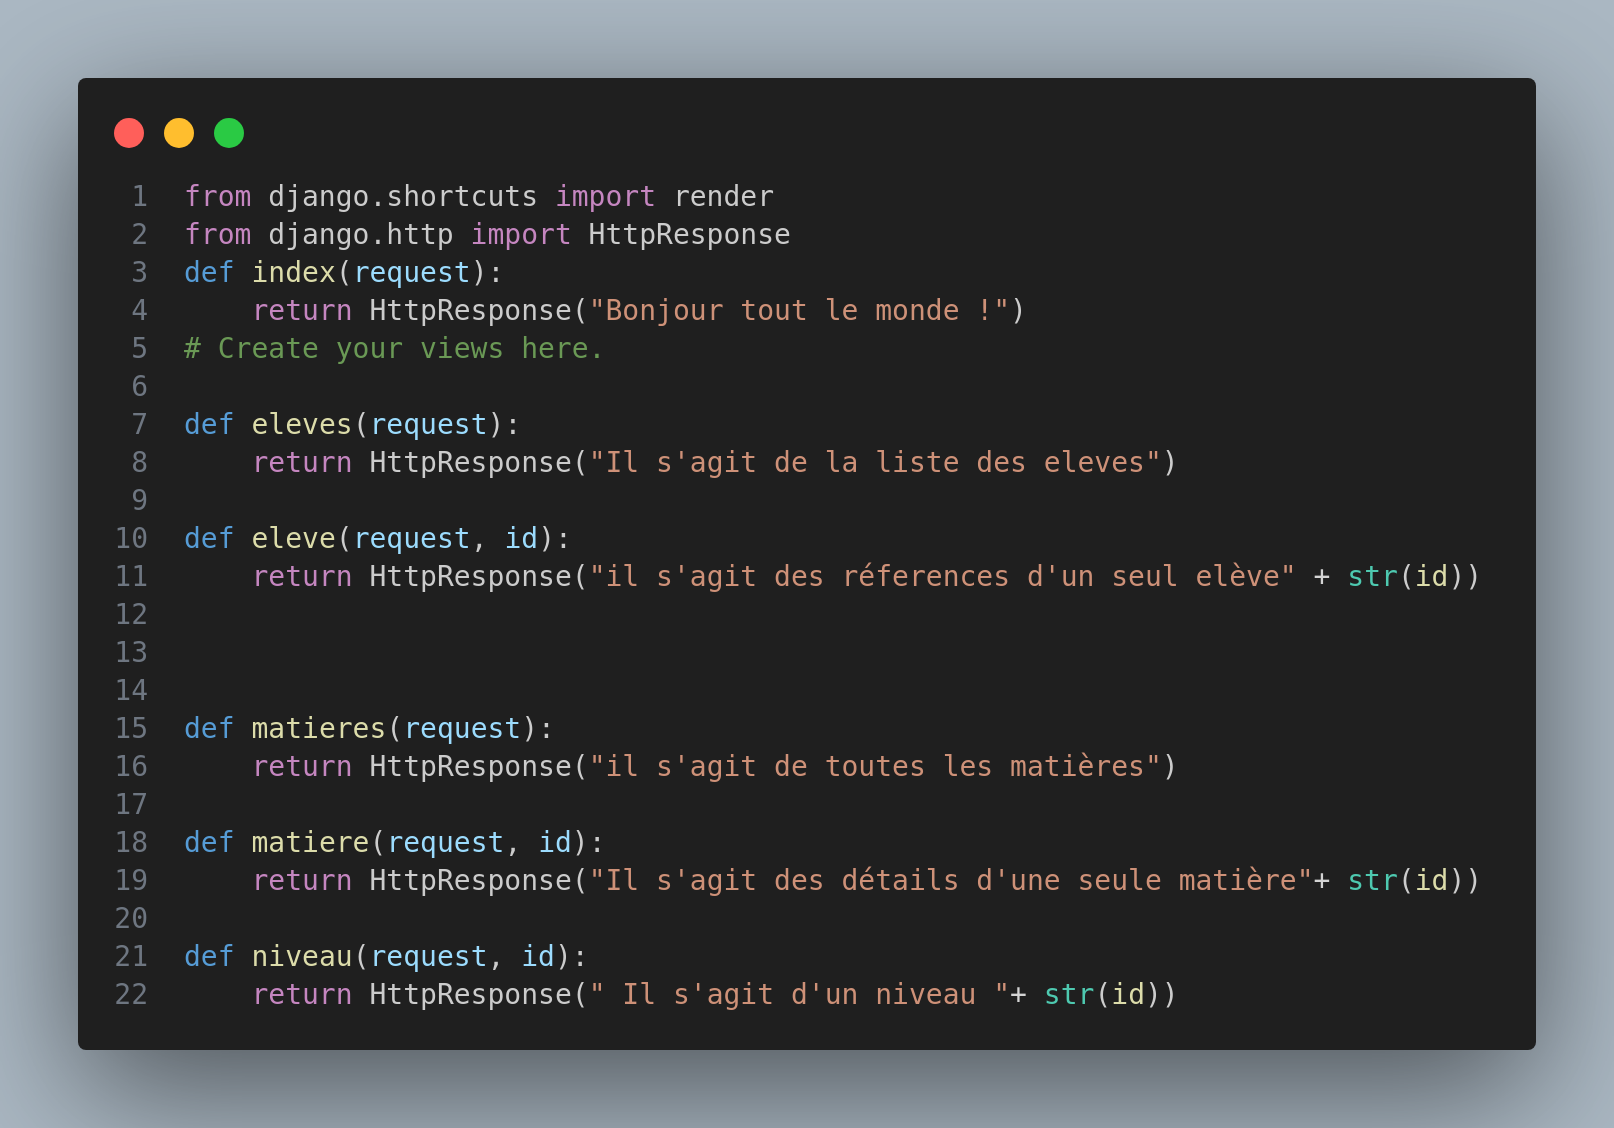
\includegraphics[scale=0.26]{1.png}
\end{center}

\item Pour que ces vues soient accessible il il faut que je définisse l'uri de chaque méthode contenant le chemin de la vue.
\item[•] Je vais le faire dans le fichier \textcolor{blue}{urls.py }

%Ne pas oublier de lire la \href{http://texnique.fr/osqa/faq/}{FAQ de \TeX nique}.

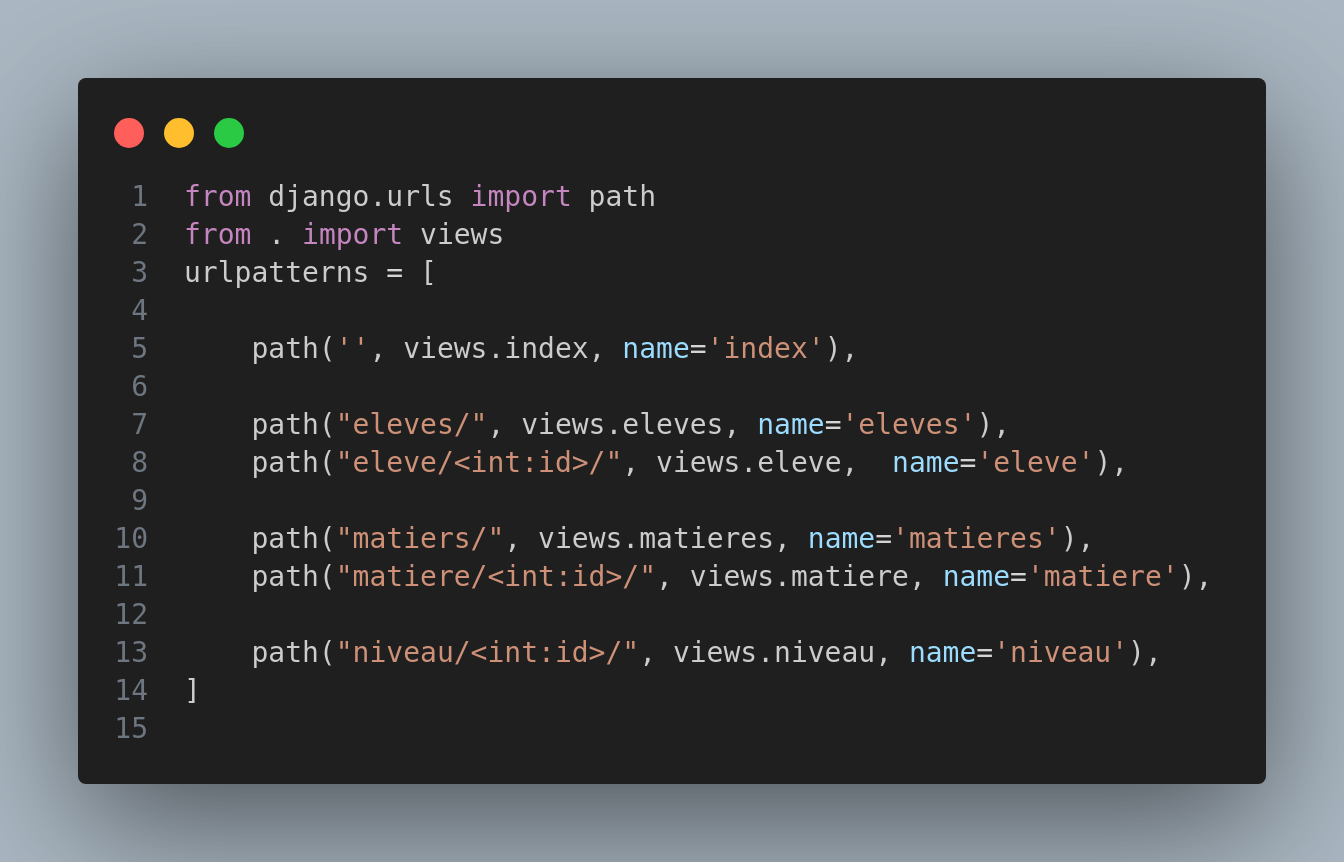
\includegraphics[scale=0.31]{2.png}
\item Pour accéder a la page de détails : \\
\_Je prend pour exemple pour élève donc j'ai fais :\\ \textcolor{blue}{http://localhost:8000/notes/eleve/2/}\\
\_Pour matière : \\ \textcolor{blue}{http://localhost:8000/notes/matiere/1/}

\item Les modèles qui doivent êtres appelés pour chacune des vues : modèles élève, matière, niveau.\\
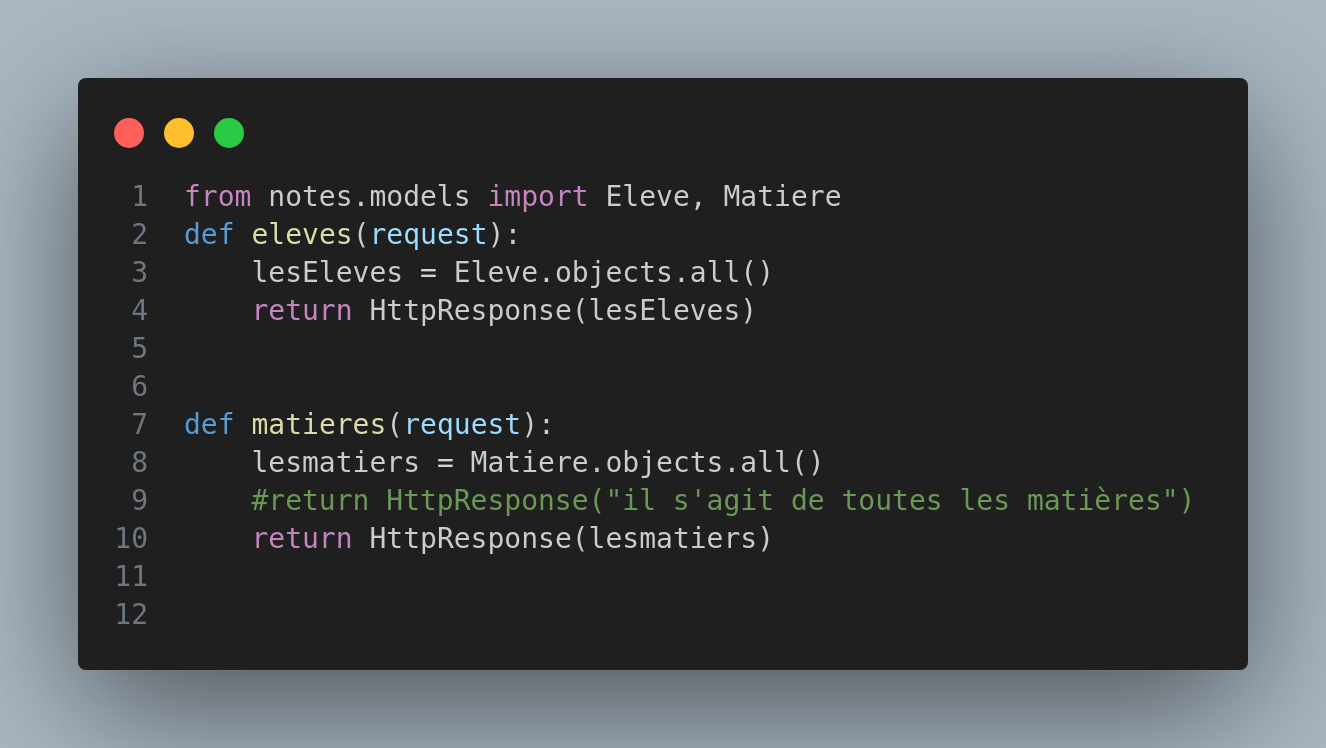
\includegraphics[scale=0.29]{3.png}
\end{enumerate}


\section{Les templates}
\begin{enumerate}
\item Un template est un moteur de rendue de données.
\item Ce code ne vas rien faire.
\item La fonction \textcolor{blue}{render} permet de retourner un template. 

\item Report du code .\\packet tracr 1.5.7
\begin{center}
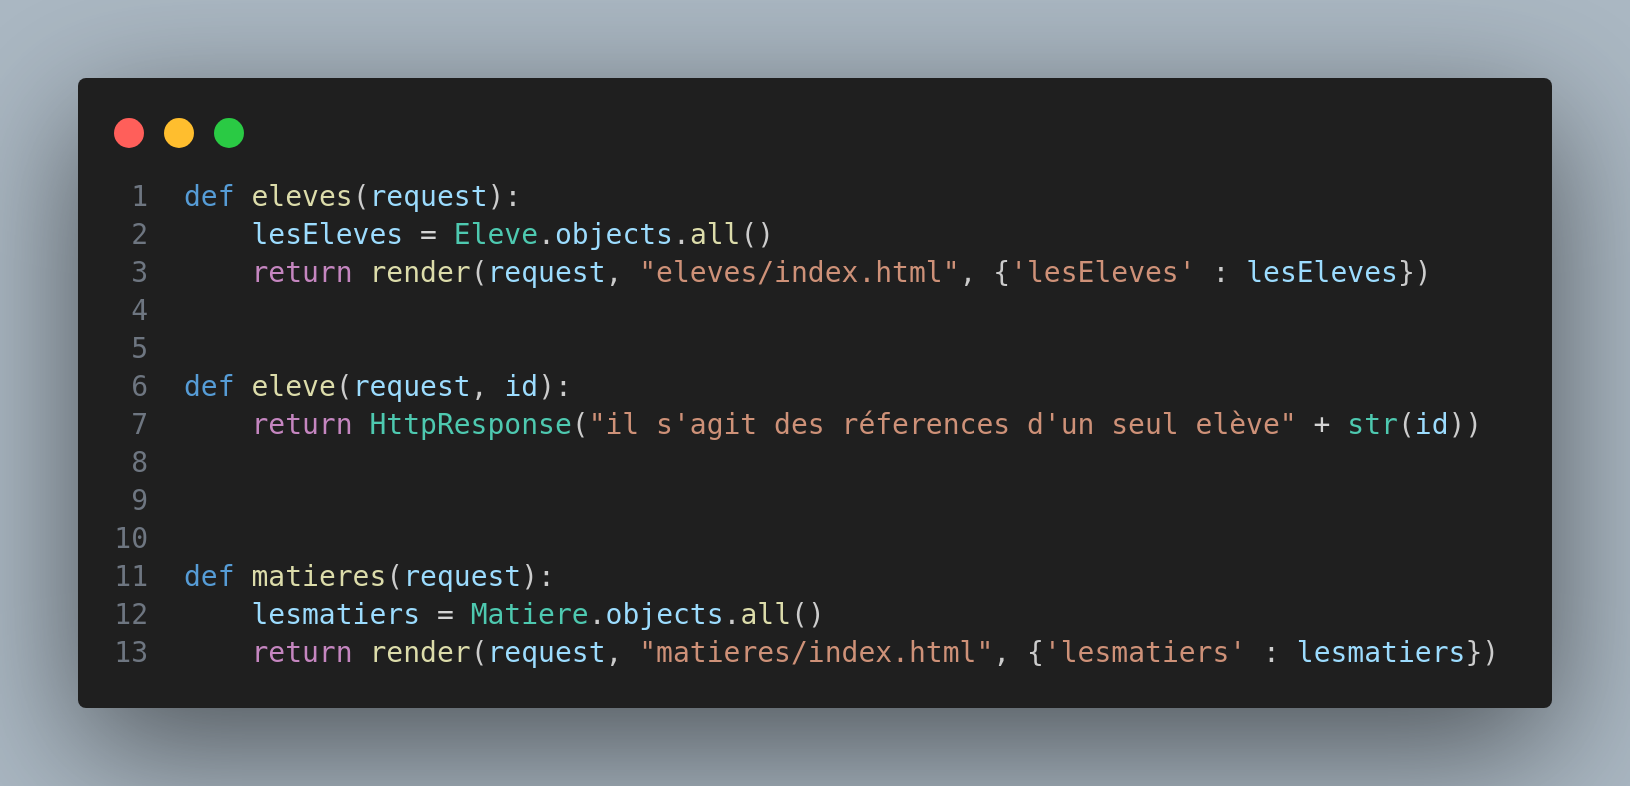
\includegraphics[scale=0.23]{4.png}
\end{center}

Contenu des fichier matiere/index.html et eleves/index.html\\

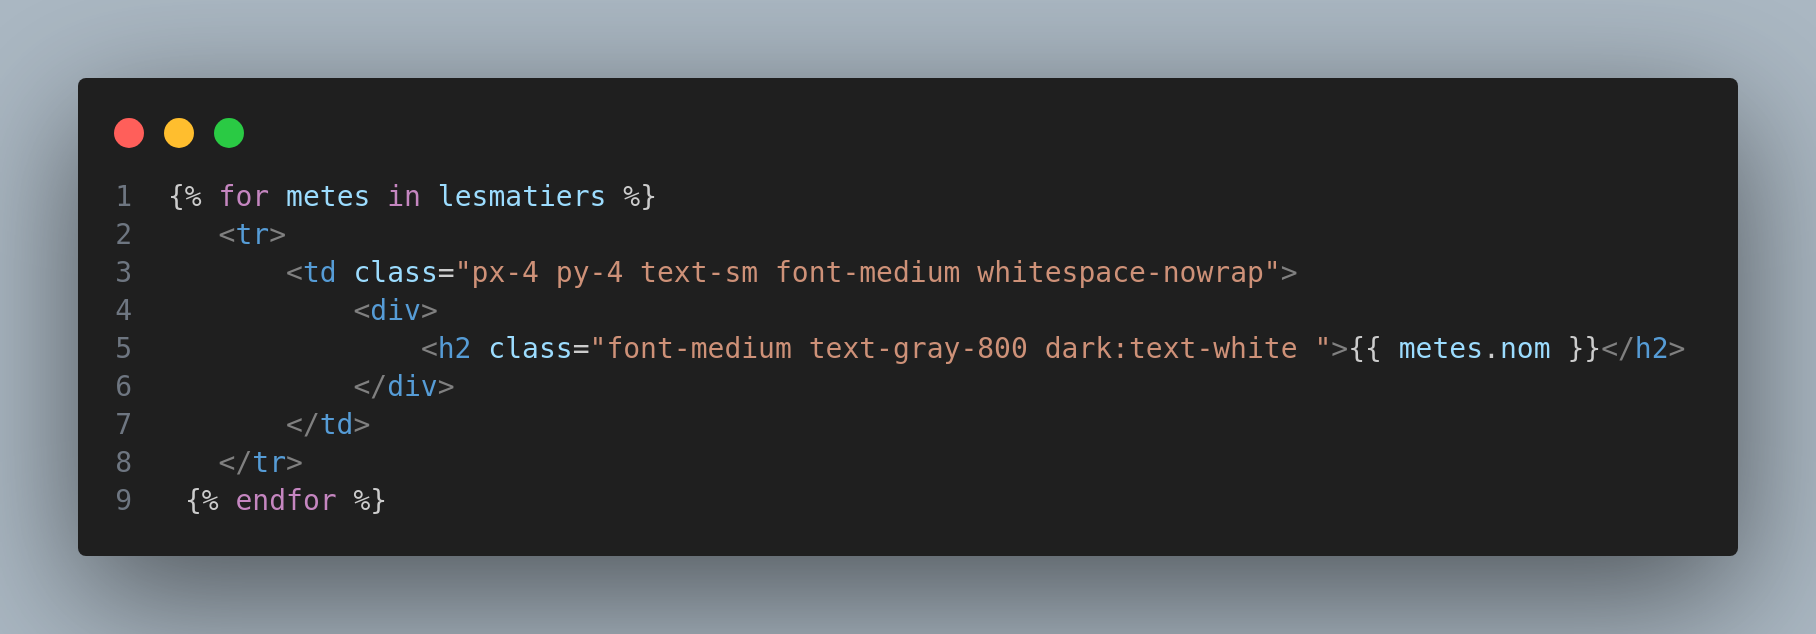
\includegraphics[scale=0.21]{5.png}
\end{enumerate}

\section{Gestion des erreurs}
\begin{enumerate}
\item Les autres vues sont différents parce qu'elles comportent des paramètre.
\item La fonction \textcolor{blue}{get\_object\_or\_404} appelle get() d’un gestionnaire de modèle donné, mais génère une exception Http404 au lieu de l’exception DoesNotExist du modèle.\\\\
Cette fonction nous sera utile dans les autres vues pour la simple raison que si on retourne une vue qui n'existe pas alors on aura une erreur 404. 

\item Architecture du templates\\\\
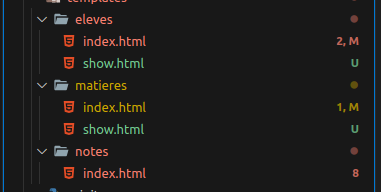
\includegraphics[scale=0.8]{6.png}

\_Contenu du fichier views.py\\

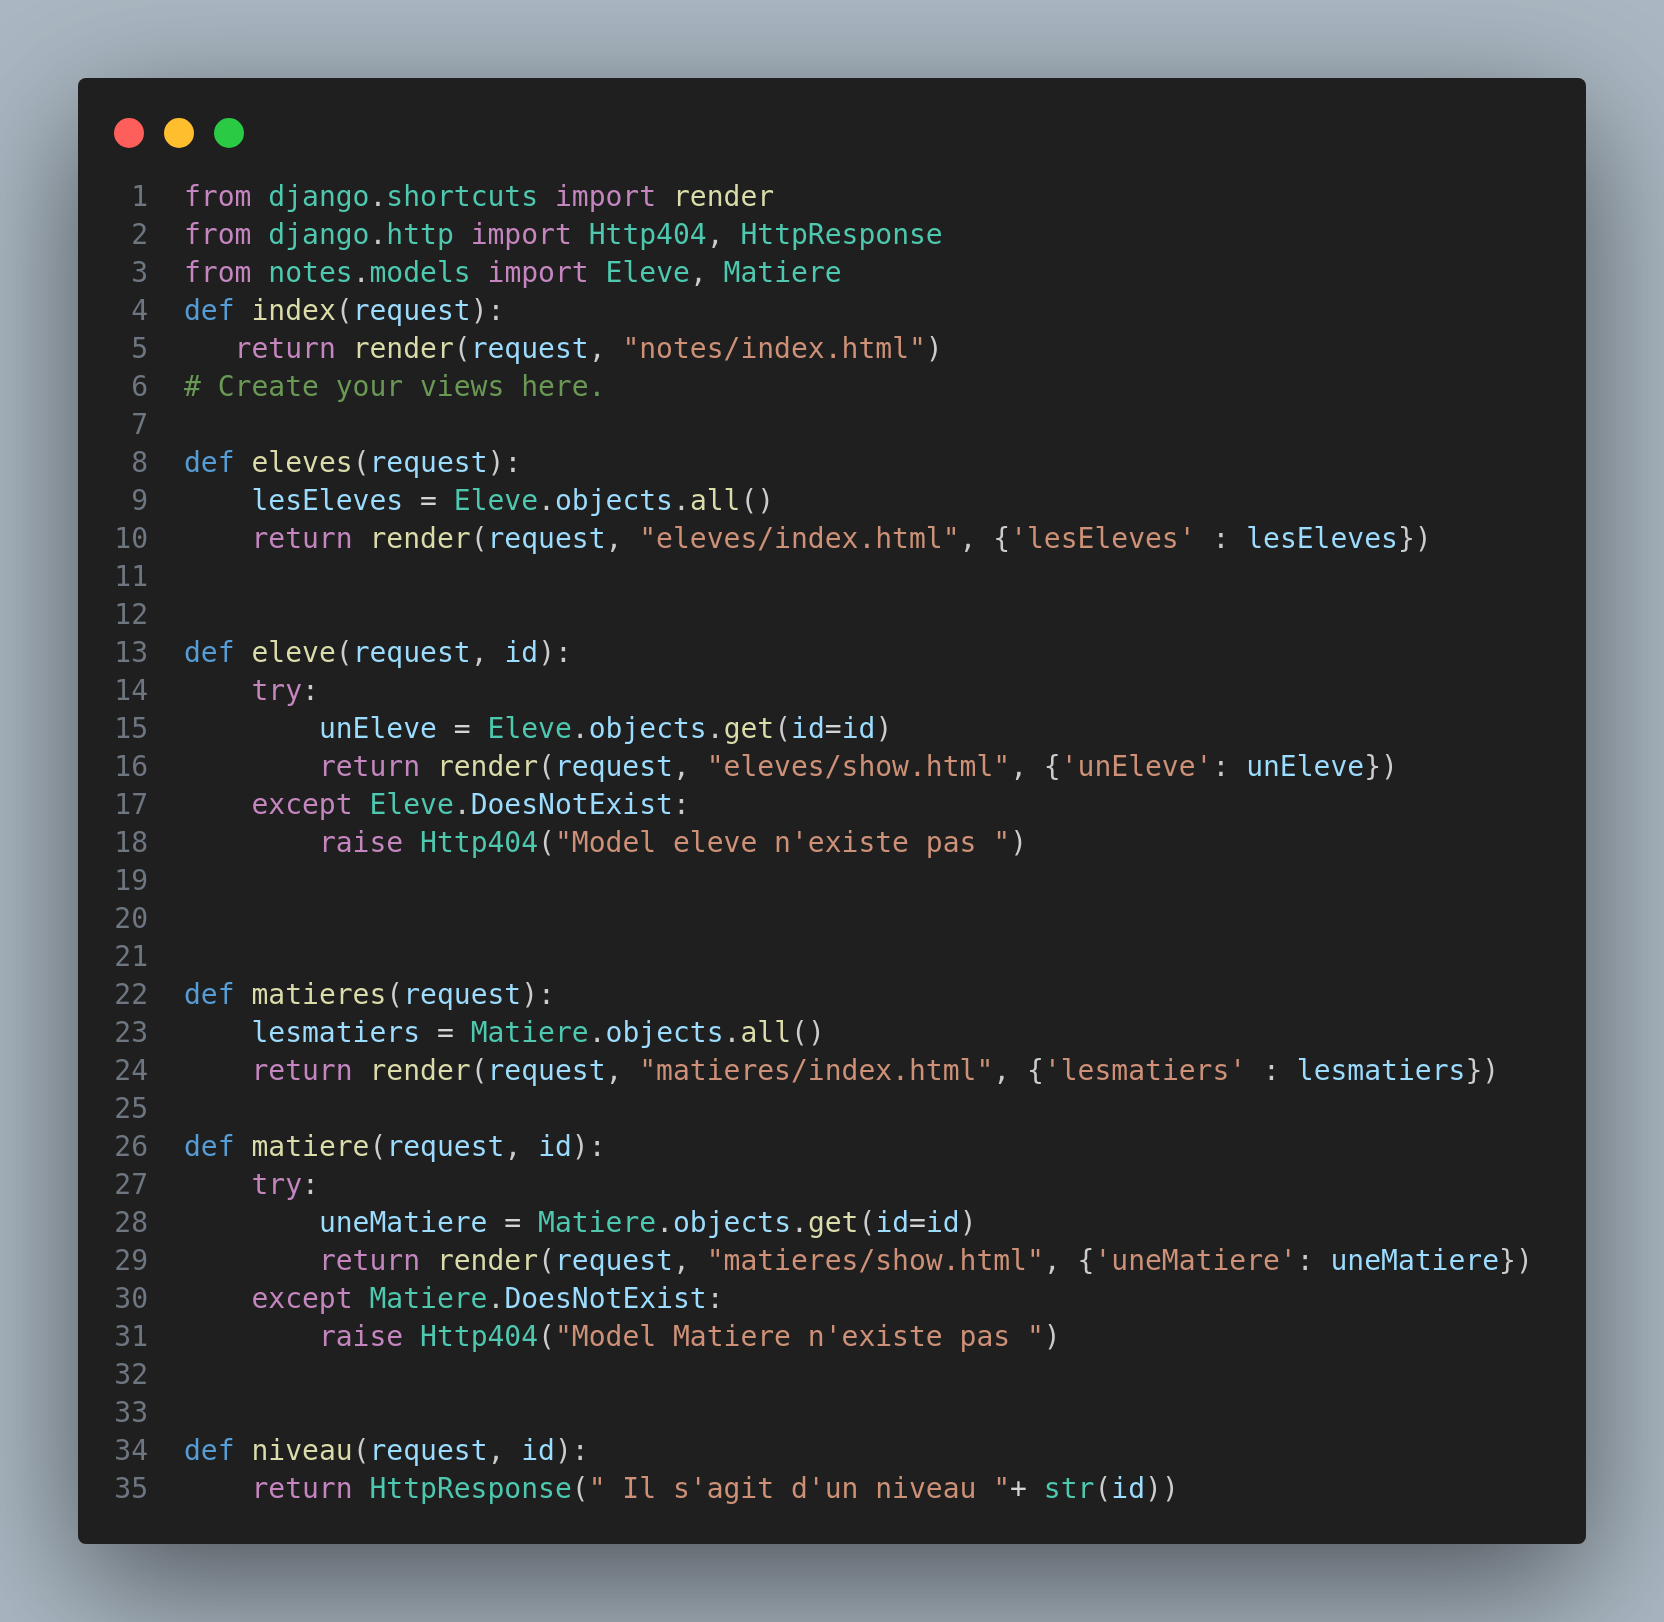
\includegraphics[scale=0.2]{9.png}

\item La ligne de code qu'on doit supprimer\\ \textcolor{blue}{from django.http import HttpResponse}
\end{enumerate}


\section{Navigation et espaces de noms}
\begin{enumerate}
\item Reporte de tous les templates\\
\begin{center}
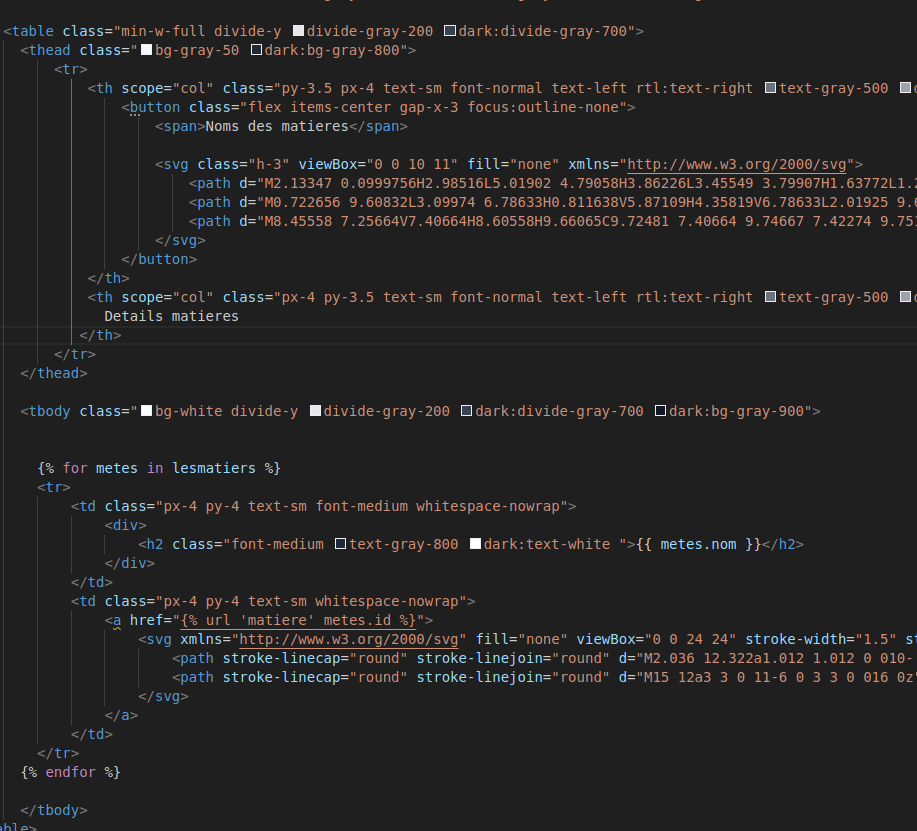
\includegraphics[scale=0.4]{tab.png}
\end{center}

\item Pour les améliorer nous devons ajouter du style pour une meilleur visibilité.

\item Différence entre un projet et une application. Une application est un ensemble d'application. Et une application est un programme exécutant certaines actions donnée.
\item[•] Un projet encapsule une application.
\item[•] Dans notre TP notes correspond a une application.


\item En django il est possible de créer un nombre incalculable d'application.

\begin{center}
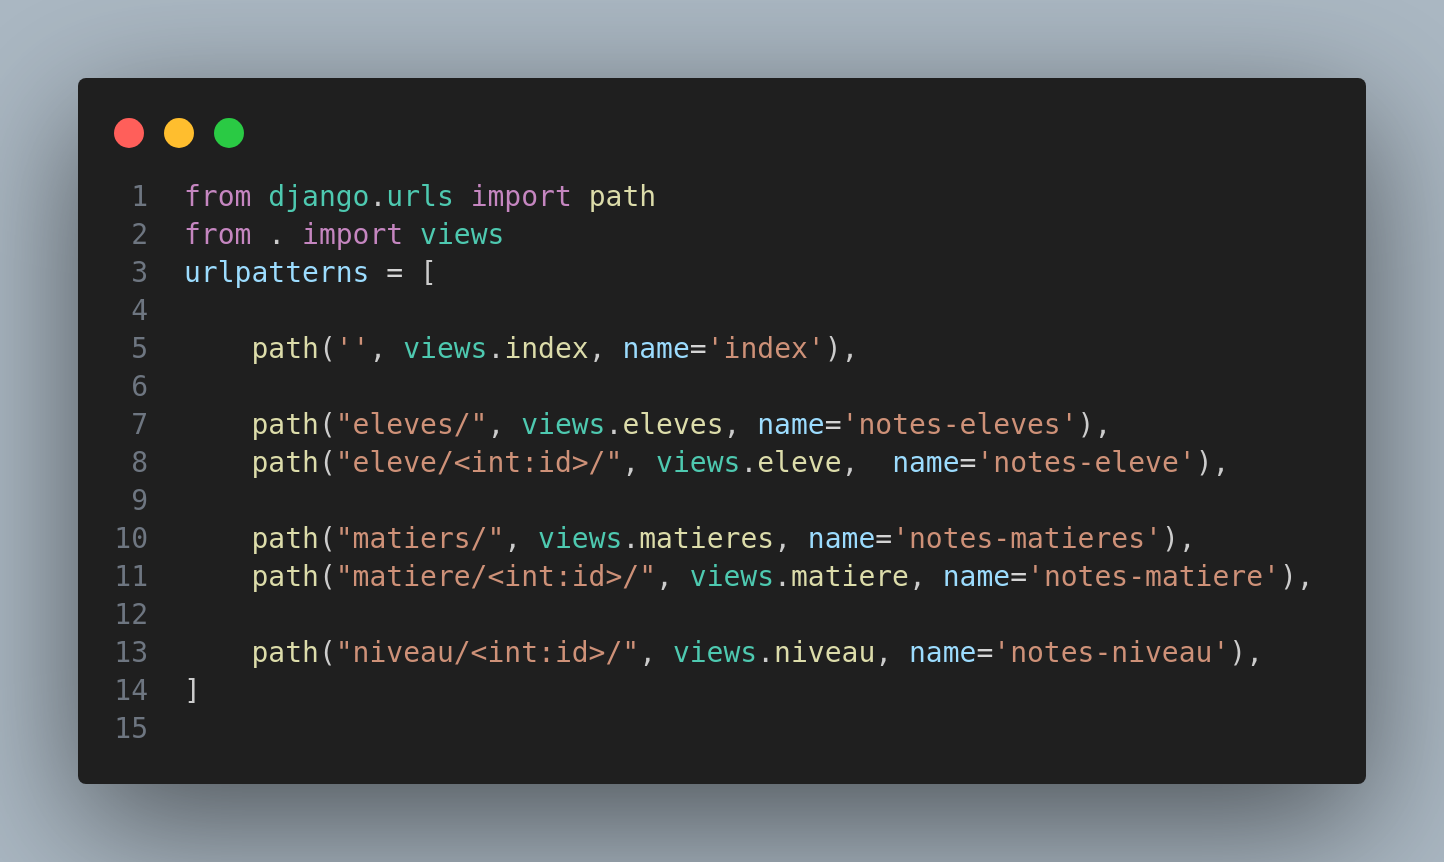
\includegraphics[scale=0.3]{10.png}
\end{center}






\end{enumerate}













\end{document}